\documentclass{beamer}
\usetheme{Madrid}

\AtBeginSection[]{
  \begin{frame}
  \vfill
  \centering
  \begin{beamercolorbox}[sep=8pt,center,shadow=true,rounded=true]{title}
    \usebeamerfont{title}\insertsectionhead\par%
  \end{beamercolorbox}
  \vfill
  \end{frame}
}


\usepackage{amsmath}
\usepackage{amssymb}
\usepackage{amsthm}
\usepackage{multicol}
\theoremstyle{remark}
\newtheorem{remark}{Remark}
\usepackage{mathtools}
\usepackage[]{graphicx}
\usepackage{libertinus}
\usepackage{caption}
\usepackage{subcaption}
\usepackage[backend=biber]{biblatex}
\addbibresource{bibliography.bib}

\newcommand{\gammabf}{\boldsymbol{\gamma}}
\newcommand{\Gammabf}{\boldsymbol{\Gamma}}
\newcommand{\const}{\, \text{const.}}
\newcommand{\xbf}{\mathbf{x}}
\newcommand{\ybf}{\mathbf{y}}
\newcommand{\intd}{\, \text{d}}
\newcommand{\norm}[1]{\lvert \lvert #1 \rvert \rvert}
\newcommand{\inner}[1]{\langle \langle #1 \rangle \rangle}

\DeclareMathOperator{\grad}{grad}
\DeclareMathOperator{\dist}{dist}
\DeclareMathOperator{\laplace}{\Delta}

\setlength{\columnseprule}{1pt}


\title{Untangling Knots Through Curve Repulsion}
\titlegraphic{
\includegraphics[height=2cm]{oxfordlogo.eps}}
\author{Joo-Hyun Paul Kim}

\begin{document}

% Title Page
\begin{frame}
    \titlepage
\end{frame}

\begin{frame}
    \frametitle{What the curious folks ponder about}
    \tableofcontents
\end{frame}

\section{Introduction}
\begin{frame}
    \frametitle{A Cool Knot}
    \begin{figure}[h]
        \centering
        \includegraphics[scale=0.25]{knot}
        \caption{Imagine your earphones getting tangled like this\ldots}
    \end{figure}
\end{frame}


\begin{frame}
    \frametitle{Aim}
    \begin{itemize}
        \item<1-> Finding a ``homotopy'' from a knot to an unknot.
            \begin{figure}[h]
                \centering
                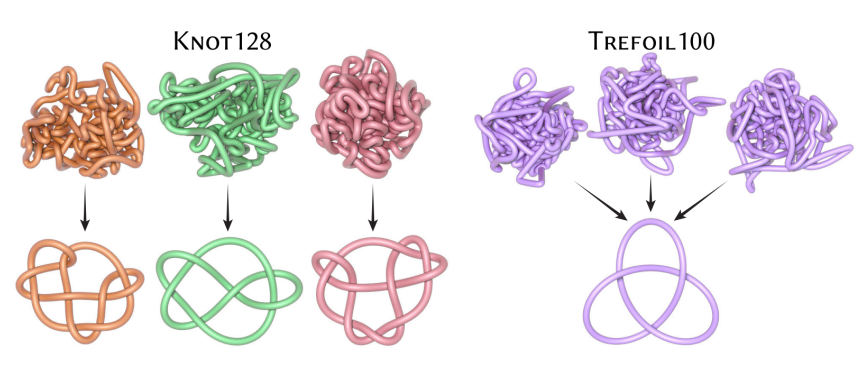
\includegraphics[scale=0.2]{knotsolving}
                \caption{Unknots of test knots.\cite{YSC2021}}
            \end{figure}
        \item<2-> ``Avoiding self-intersection''
    \end{itemize}
\end{frame}

\begin{frame}
    \frametitle{General Strategy}
    \begin{enumerate}
        \item<1-> Define curve energy; penalizing the closeness of points on a curve.
            \begin{itemize}
                \item Extreme-closeness of points on curve is a natural characteristic of a tangled curve.
            \end{itemize}
        \item<2-> Attempt to decrease the curve energy by continuously deforming the curve.
            \begin{itemize}
                \item We evolve the curve according to the gradient flow equation.
                \item There is a freedom in choosing the ``gradient'' here.
            \end{itemize}
        \item<3-> We expect the stationary state to be the ``unknot''
            \begin{itemize}
                \item Or at least a simpler state\ldots
            \end{itemize}
    \end{enumerate}

\end{frame}

\section{Tangent-Point Energy}
\begin{frame}
    \frametitle{Defining Curve Energy}
    \onslide<1->{
        Given an (arc-length parameterised) curve $\gammabf:M \rightarrow \mathbb{R}^3$, we wish to assign energy of the form:
        \begin{equation}
            \mathcal{E} \left( \gammabf \right) \coloneqq \iint_{M^2} k \left( \gammabf_x, \gammabf_y \right) \intd \gamma_x \intd \gamma_y
        \end{equation}
        such that
        \begin{itemize}
            \item $\mathcal{E}$ is very high when two non-neighbouring points are very close.
        \end{itemize}
    }
    \onslide<2>{
        A na\"ive choice is $k \left( \gammabf_x, \gammabf_y \right) \coloneqq \frac{1}{\norm{\gammabf_x - \gammabf_y}}$
    }
\end{frame}

\begin{frame}
    \frametitle{Pitfall of the ``Simple Energy''}
        \begin{equation*}
            \mathcal{E} \left( \gammabf \right) \coloneqq \iint_{M^2} \frac{1}{\norm{\gammabf_x - \gammabf_y}} \intd \gamma_x \intd \gamma_y
        \end{equation*}
        \begin{figure}[h]
            \centering
            \begin{subfigure}[b]{0.45\textwidth}
                \centering
                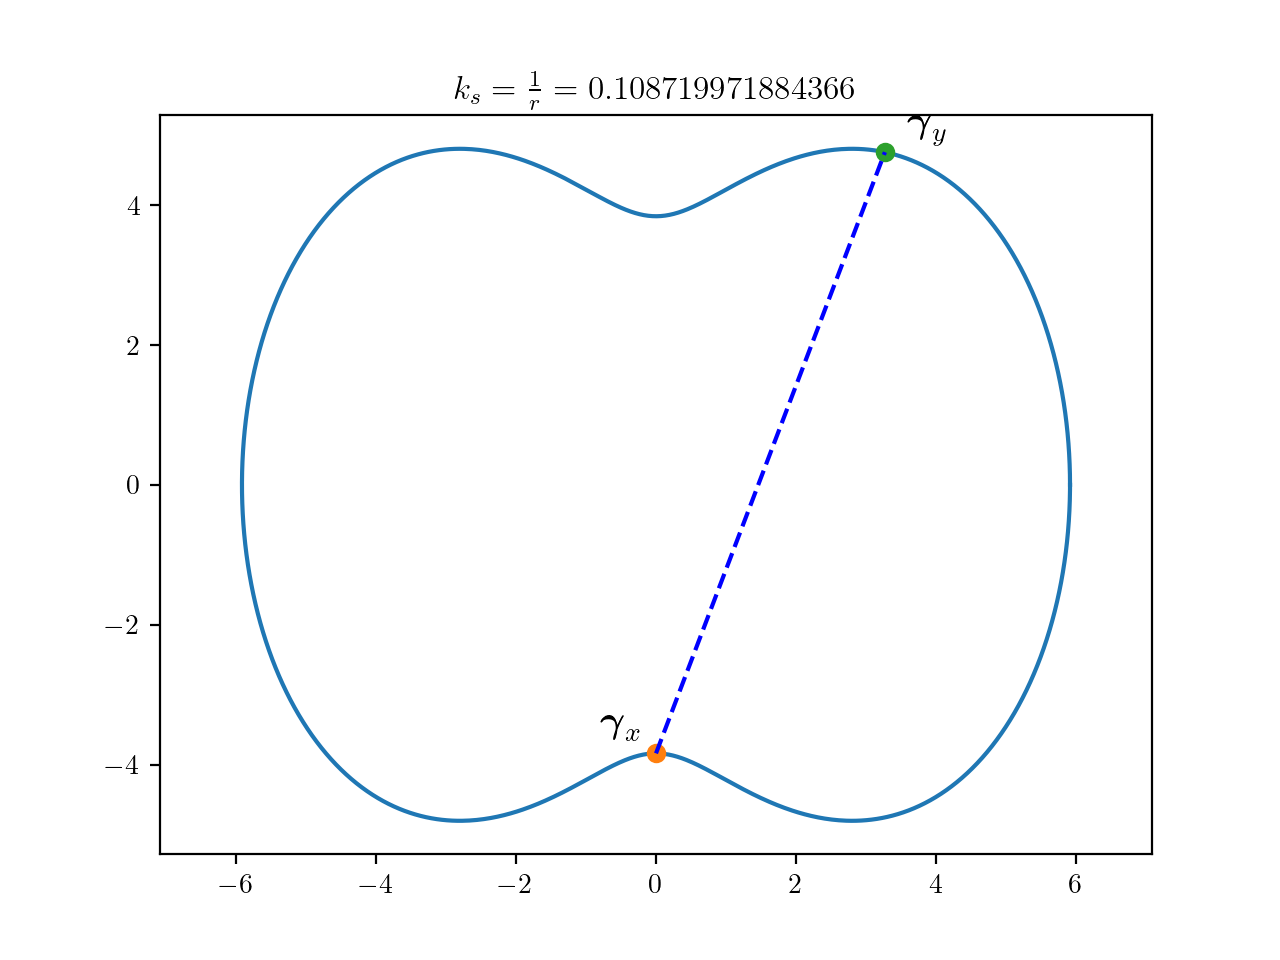
\includegraphics[width=\textwidth]{simple-0}
            \end{subfigure}
            \begin{subfigure}[b]{0.45\textwidth}
                \centering
                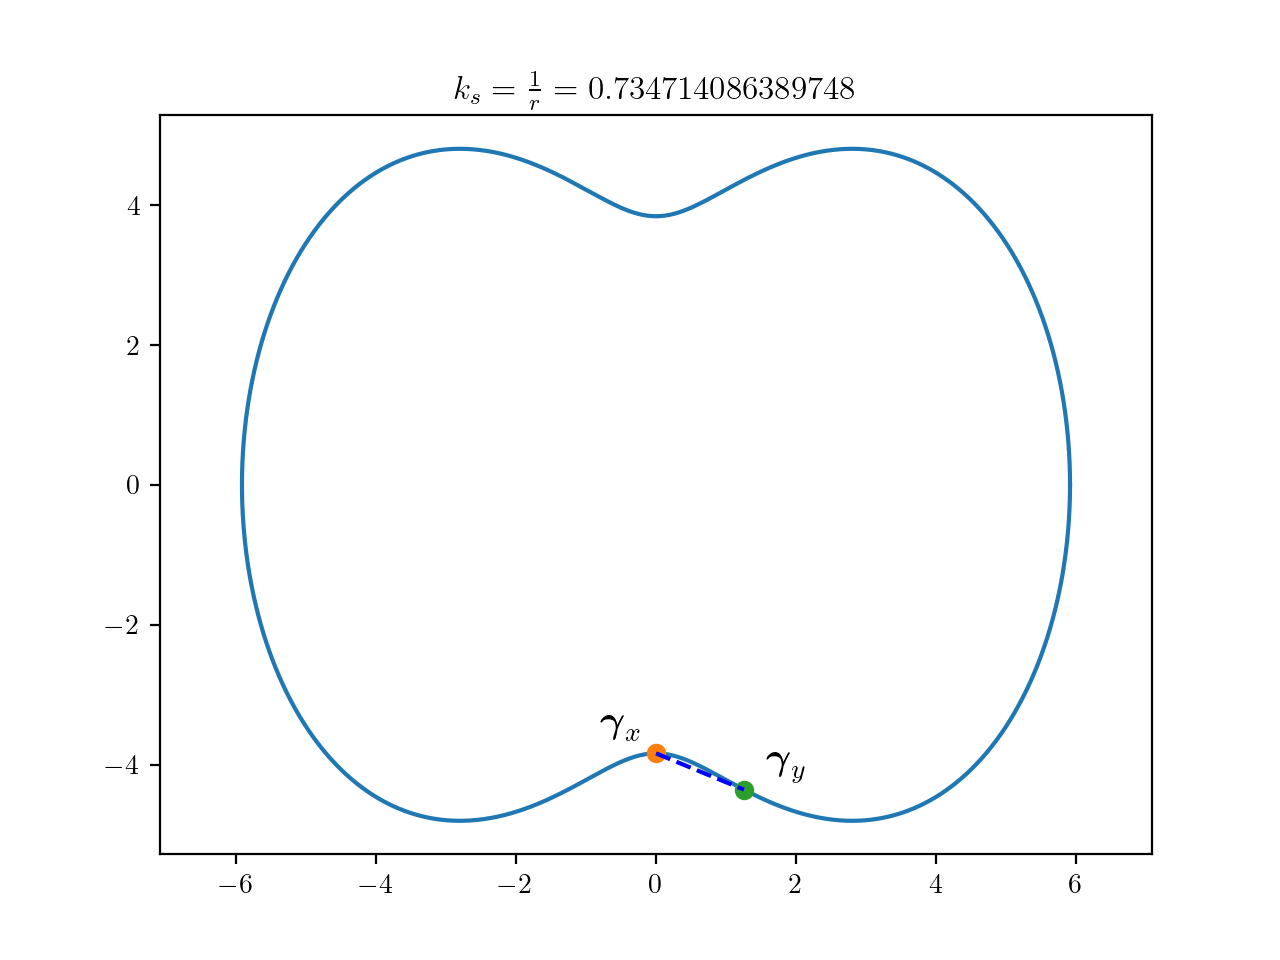
\includegraphics[width=\textwidth]{simple-1}
            \end{subfigure}
        \end{figure}
\end{frame}

\begin{frame}
    \frametitle{Pitfall of the ``Simple Energy''}
        \begin{equation*}
            \mathcal{E} \left( \gammabf \right) \coloneqq \iint_{M^2} \frac{1}{\norm{\gammabf_x - \gammabf_y}} \intd \gamma_x \intd \gamma_y
        \end{equation*}
        \begin{figure}[h]
            \centering
            \begin{subfigure}[b]{0.45\textwidth}
                \centering
                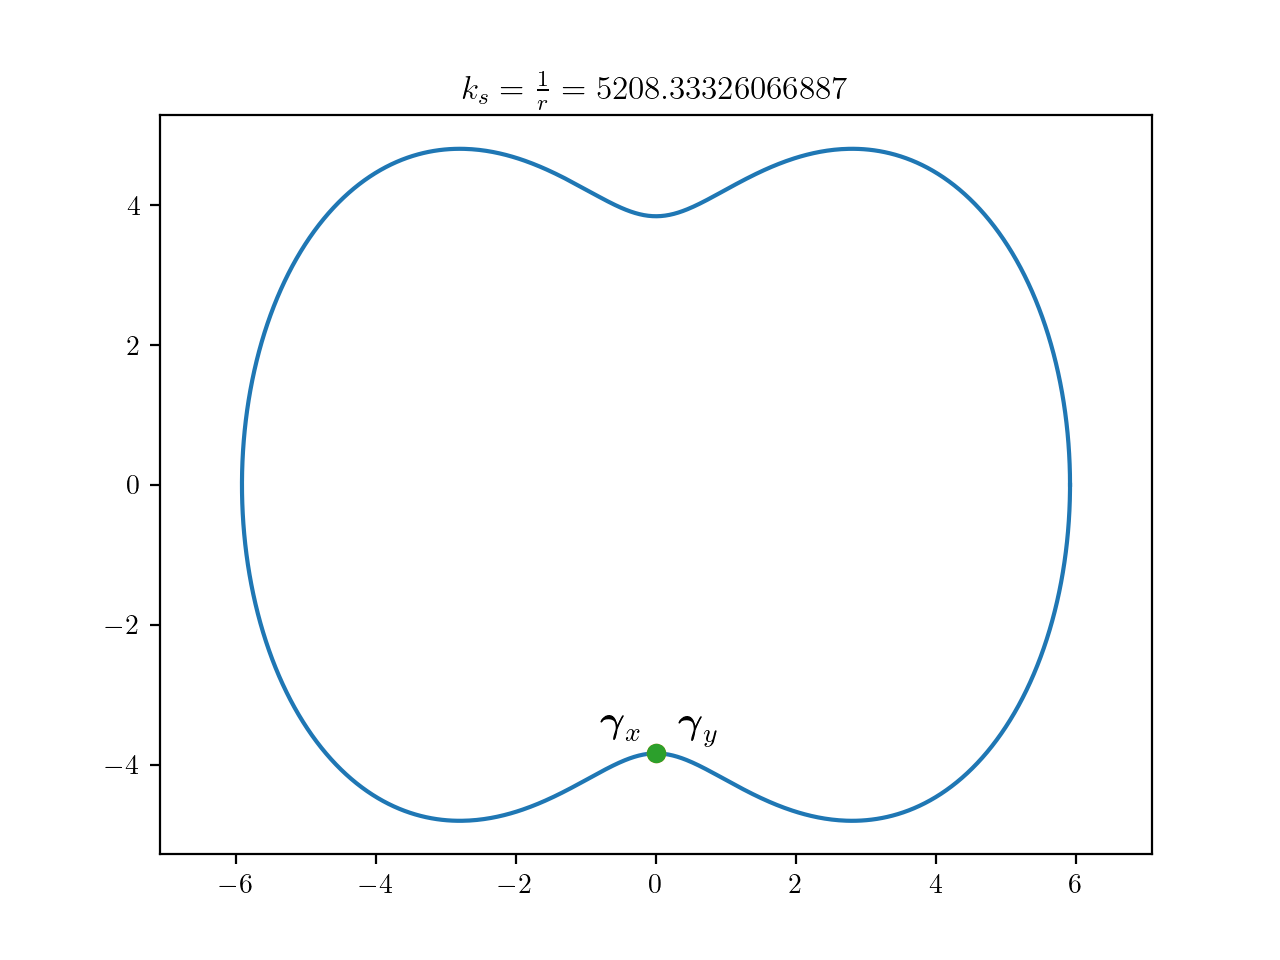
\includegraphics[width=\textwidth]{simple-2}
            \end{subfigure}
            \begin{subfigure}[b]{0.45\textwidth}
                \centering
                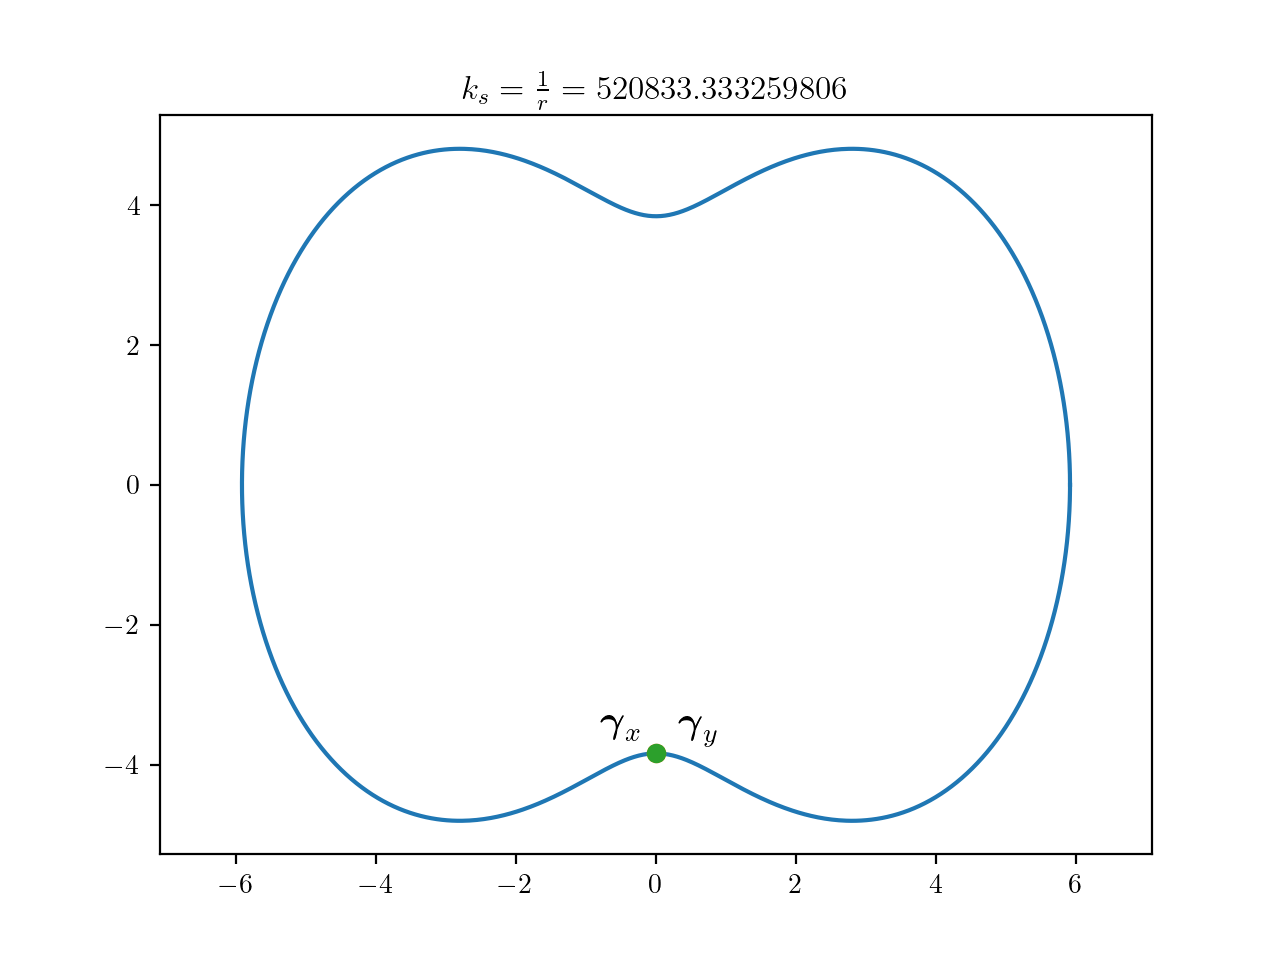
\includegraphics[width=\textwidth]{simple-3}
            \end{subfigure}
        \end{figure}
        \onslide<2->{
            This energy is not well-defined for a lot of curves!
        }
\end{frame}

\begin{frame}
    \frametitle{Buck-Orloff Tangent-Point Energy}
    \begin{itemize}
        \item From the simple energy, need a way to suppress the infinite contribution of the ``singularity''.
    \end{itemize}
    \begin{definition}[Buck-Orloff Tangent-Point Energy]<2->
        For a smooth curve $\gammabf$, define
        \begin{equation*}
            \mathcal{E} \left( \gammabf \right) \coloneqq \iint_{M^2} k_{4}^2 \left( \gammabf_x, \gammabf_y, \mathbf{T}_x \right) \intd \gamma_x \intd \gamma_y
        \end{equation*}
        where $\mathbf{T}_x$ is the unit tangent vector at $\gammabf_x$,
        with the kernel defined as
        \begin{equation*}
            k_4^2 \left( \mathbf{p}, \mathbf{q}, \mathbf{T} \right) \coloneqq \frac{\norm{\mathbf{T} \wedge \left( \mathbf{p} - \mathbf{q} \right)}^{2}}{\norm{\mathbf{p} - \mathbf{q}}^{4}}
        \end{equation*}
        as \textbf{Buck-Orloff Tangent-Point Energy}.\cite{BO1995}
    \end{definition}
\end{frame}

\begin{frame}
    \frametitle{Intuition}
    What is the intuition behind the kernel $k_4^2 \left( \mathbf{p}, \mathbf{q}, \mathbf{T} \right) \coloneqq \frac{\norm{\mathbf{T} \wedge \left( \mathbf{p} - \mathbf{q} \right)}^{2}}{\norm{\mathbf{p} - \mathbf{q}}^{4}}$?

    \onslide<2->
    {
        \begin{figure}[h]
            \centering
            \begin{subfigure}[b]{0.48\textwidth}
                \centering
                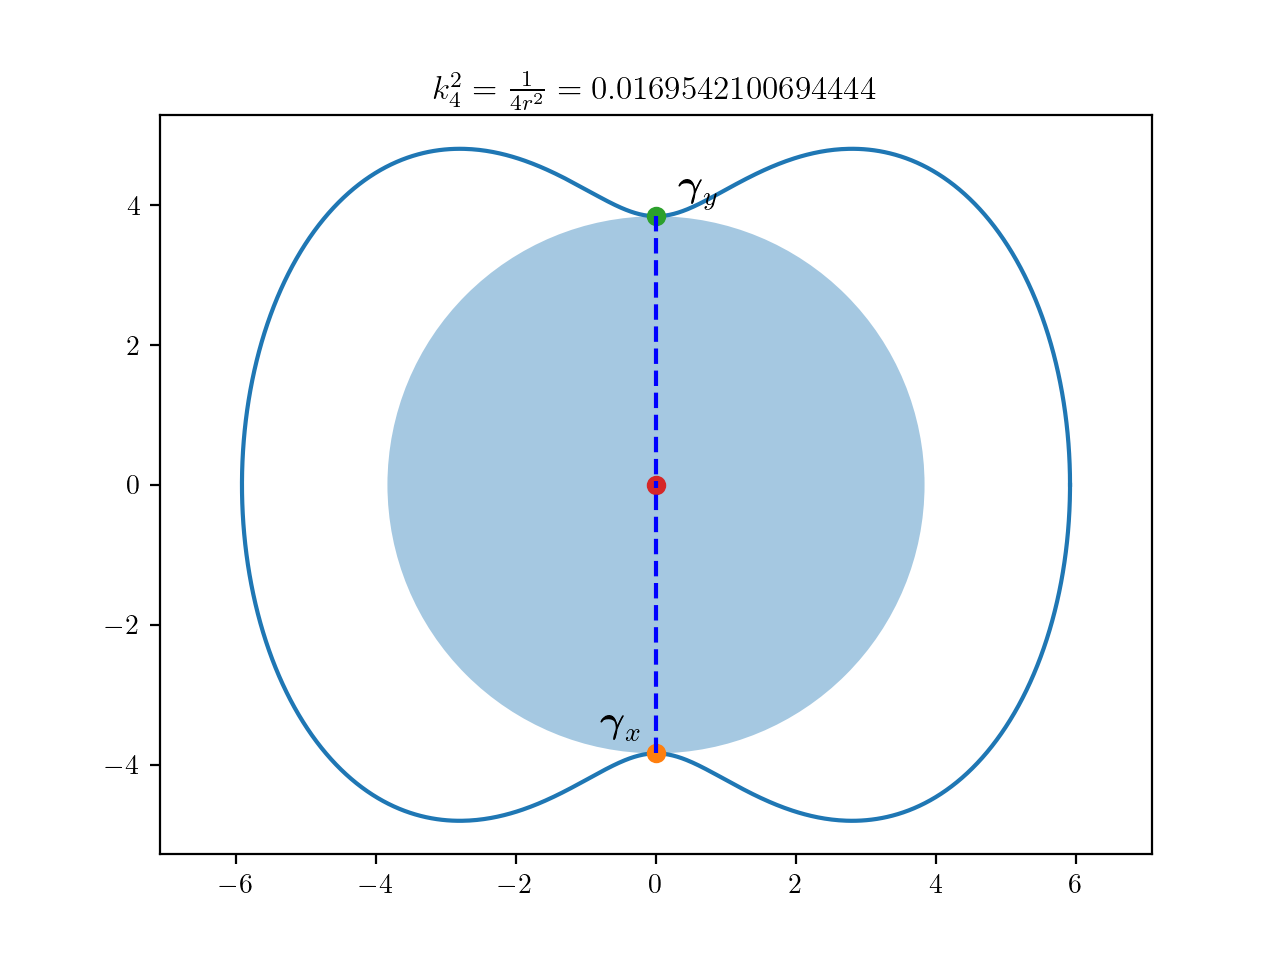
\includegraphics[width=\textwidth]{straight}
            \end{subfigure}
            \begin{subfigure}[b]{0.48\textwidth}
                \centering
                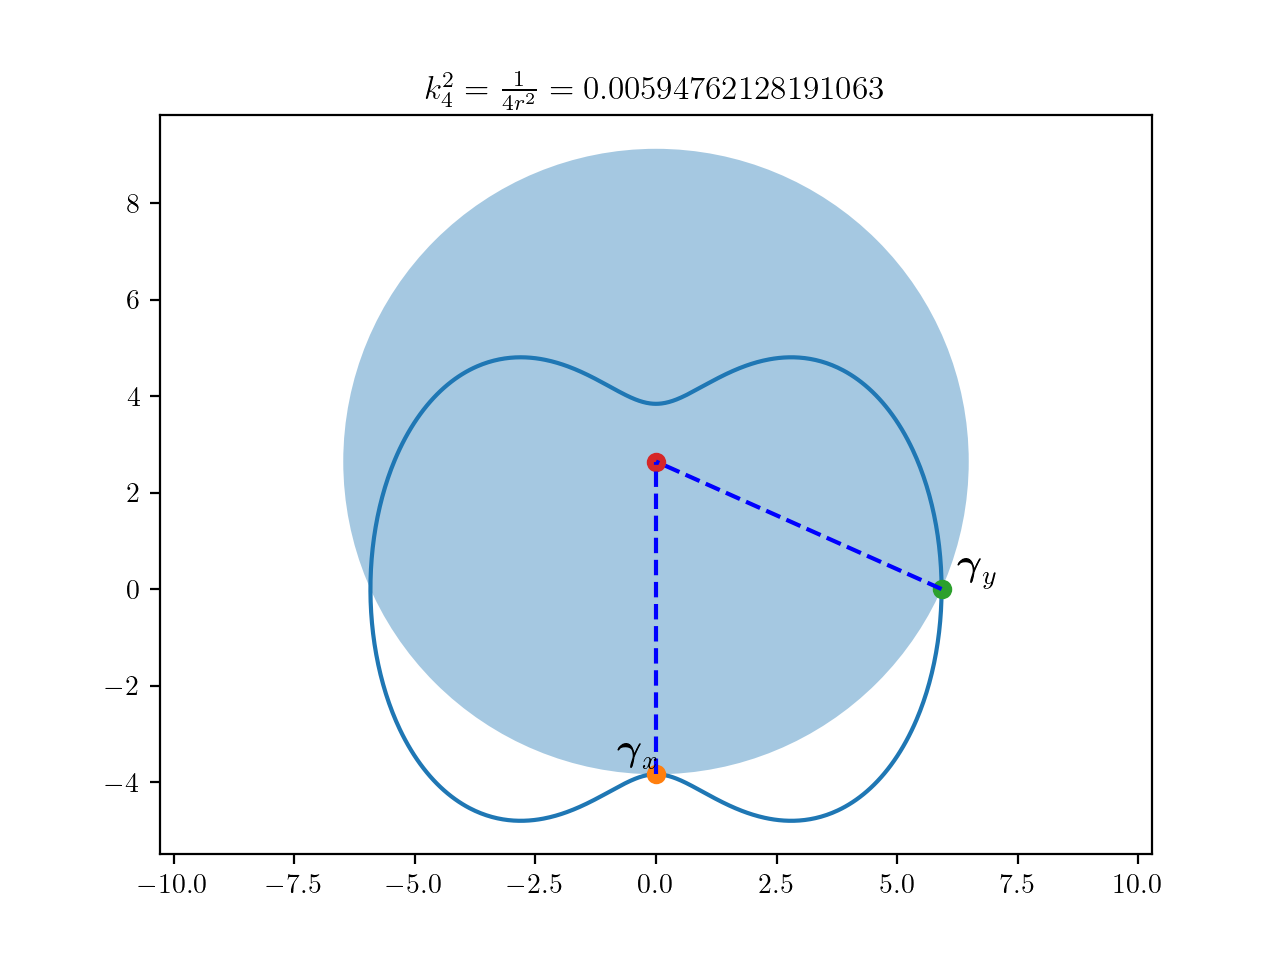
\includegraphics[width=\textwidth]{0}
            \end{subfigure}
        \end{figure}
    }

    \begin{remark}<3->
        Note that closer does not necessarily mean the kernel is larger.
    \end{remark}
\end{frame}

\begin{frame}
    \frametitle{Intuition}
    \begin{figure}[h]
        \centering
        \includegraphics[scale=0.5]{perturbed}
        \caption{When two points are very close, the kernel converges to the curvature of the curve.}
    \end{figure}
\end{frame}

%\begin{frame}
%    \frametitle{Example: Buck-Orloff Tangent-Point Energy of a Circle}
%    \begin{example}
%        Suppose we wish to compute the Buck-Orloff tangent-point energy of a unit circle.
%        \onslide<2->
%        {
%            Parameterise unit circle as:
%            \begin{multicols}{2}
%            \begin{equation*}
%                \gammabf (t) = \left( \cos{t}, \sin{t}, 0 \right)
%            \end{equation*}
%            \columnbreak
%            \begin{figure}[h]
%                \centering
%                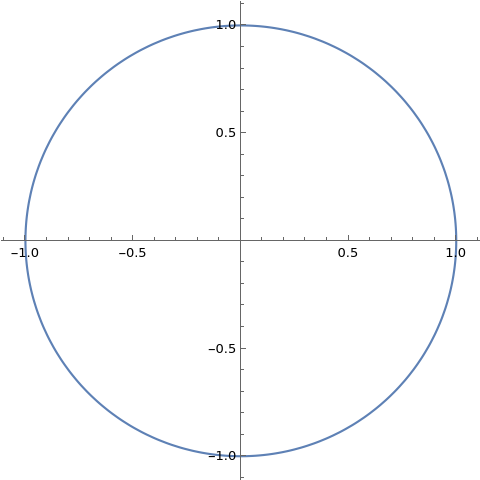
\includegraphics[scale=0.2]{unitcircle}
%            \end{figure}
%            \end{multicols}
%        }
%        \onslide<3->
%        {
%            Then write:
%            \begin{equation*}
%                \begin{cases}
%                    \gammabf_x \left( \theta \right) = \left( \cos{\theta}, \sin{\theta}, 0 \right) \\
%                    \gammabf_y \left( \phi \right) = \left( \cos{\phi}, \sin{\phi}, 0 \right) \\
%                    \mathbf{T}_x \left( \theta \right) = \left( -\sin{\theta}, \cos{\theta}, 0 \right)
%                \end{cases}
%            \end{equation*}
%        }
%    \end{example}
%\end{frame}
%
%\begin{frame}
%    \begin{example}[Cont.]
%            \begin{equation*}
%                \begin{cases}
%                    \gammabf_x \left( \theta \right) = \left( \cos{\theta}, \sin{\theta}, 0 \right) \\
%                    \gammabf_y \left( \phi \right) = \left( \cos{\phi}, \sin{\phi}, 0 \right) \\
%                    \mathbf{T}_x \left( \theta \right) = \left( -\sin{\theta}, \cos{\theta}, 0 \right)
%                \end{cases}
%            \end{equation*}
%            Substituting to Buck-Orloff Tangent-Point energy formula:
%        \begin{equation*}
%            \mathcal{E} \left( \gammabf \right) \coloneqq \iint_{M^2} \frac{\norm{\mathbf{T}_x \wedge \left( \gammabf_x - \gammabf_y \right)}^{2}}{\norm{\gammabf_x - \gammabf_y}^{4}} \intd \gamma_x \intd \gamma_y
%        \end{equation*}
%        \onslide<2->
%        {
%            Using a few identities:
%            \begin{align*}
%                \mathcal{E} \left( \gammabf \right) &= \int_{\theta=0}^{2 \pi} \int_{\phi=0}^{2 \pi}
%                \frac{\norm{\mathbf{T}_x}^2 \norm{\gammabf_x - \gammabf_y}^2 - \left( \mathbf{T}_x \cdot \left( \gammabf_x -\gammabf_y \right) \right)^2}{\norm{\gammabf_x - \gammabf_y}^4} \intd \theta \intd \phi
%            \end{align*}
%        }
%    \end{example}
%\end{frame}

\begin{frame}
    \begin{example}[Unit Circle]
        \begin{align}
            \mathcal{E} \left( \gammabf \right) &= \int_{\theta=0}^{2 \pi} \int_{\phi=0}^{2 \pi}
            \frac{\norm{\mathbf{T}_x}^2 \norm{\gammabf_x - \gammabf_y}^2 - \left( \mathbf{T}_x \cdot \left( \gammabf_x -\gammabf_y \right) \right)^2}{\norm{\gammabf_x - \gammabf_y}^4} \intd \theta \intd \phi \\
            &= \int_{\theta=0}^{2 \pi} \int_{\phi=0}^{2 \pi}
            \frac{\sin^2 \frac{\theta - \phi}{2}}{\left( -1 + \cos \left( \theta - \phi \right) \right)^2} \intd \theta \intd \phi \\
            &= \int_{\theta=0}^{2 \pi} \int_{\phi=0}^{2 \pi}
            \frac{\sin^2 \frac{\theta - \phi}{2}}{\sin^4 \frac{\theta - \phi}{2}} \intd \theta \intd \phi
            \label{equ: 1 over r squared order}
            \\
            &= \pi^2
        \end{align}
    \end{example}
    \begin{remark}<2->
        Note that (\ref{equ: 1 over r squared order}) suggests the order at ``singularity'' is inverse-square.
    \end{remark}
\end{frame}

\begin{frame}
    \frametitle{General Tangent-Point Energy}
    A more general form of tangent-point energy comes from Yu, Schumacher, and Crane \cite{YSC2021}:
    \begin{definition}[Generalised Tangent-Point Energy]
        \begin{equation*}
            \mathcal{E}_{\beta}^{\alpha} \left( \gammabf \right) \coloneqq
            \iint_{M^2} \frac{\norm{\mathbf{T}_x \wedge \left( \gammabf_x - \gammabf_y \right)}^{\alpha}}{\norm{\gammabf_x - \gammabf_y}^{\beta}}
            \intd \gamma_x \intd \gamma_y
        \end{equation*}
        where $\alpha > 1$ and $\beta \in \left[ \alpha+2, 2\alpha+1 \right)$
    \end{definition}
    \begin{remark}
        When $\alpha = 2$ and $\beta = 4$, we are back to Buck-Orloff.
    \end{remark}
\end{frame}

\section{Gradient Flow}
%\begin{frame}
%    \frametitle{Motivating Gradient Flow}
%    A simple method of minimising a (differentiable) function $f:\mathbb{R}^n \rightarrow \mathbb{R}$ is the steepest descent \cite{doi:10.1137/1.9781611974997.ch8}
%    \begin{equation}
%        \xbf^{k+1} = \xbf^k - \alpha_k \nabla f \left( \xbf^k \right)
%    \end{equation}
%    where $\alpha^k > 0$.
%    \begin{figure}[h]
%        \centering
%        \includegraphics[scale=0.2]{sdm}
%        \caption{Steepest Descent}
%    \end{figure}
%    \onslide<2->
%    {
%        For motivation, take $\alpha^k = \alpha \equiv \const$
%    }
%\end{frame}
%
%\begin{frame}
%    \begin{equation*}
%        \xbf^{k+1} = \xbf^k - \alpha_k \nabla f \left( \xbf^k \right)
%    \end{equation*}
%    In the case of functional $\mathcal{E}: X \rightarrow \mathbb{R}$, analogously write steepest descent step:
%    \begin{equation*}
%        f^{k+1} = f^k - \alpha \grad_X f
%    \end{equation*}
%    \onslide<2->
%    {
%        Rearranging and dividing by $\Delta t$
%        \begin{equation*}
%            \frac{1}{\Delta t} \left( f^{k+1} - f^k \right) = -\alpha \grad_X f
%        \end{equation*}
%    }
%    \onslide<3->
%    {
%        Take limit as $\Delta t \rightarrow 0$, then scale time variable to nondimensionalise to get the gradient flow equation.
%        \begin{definition}[Gradient Flow Equation]
%            \begin{equation*}
%                \frac{\partial f}{\partial t} = - \grad_X f
%            \end{equation*}
%        \end{definition}
%        But what is $\grad_X f$?
%    }
%\end{frame}

\begin{frame}
    \frametitle{Motivating Gradient Flow}
    For minimising a functional $\mathcal{E}(f)$, we wish to ``move'' $f$ in the direction that decreases $\mathcal{E}$.
    \onslide<2->
    {
        \begin{definition}[Gradient Flow Equation]
            For functional $\mathcal{E} (f)$, the \textbf{gradient flow equation} is:
            $\frac{\partial f}{\partial t} = - \grad_X \mathcal{E} \left( f \right)$
        \end{definition}
    }
    \begin{remark}<3->
    cf) For minimising a function $f:\mathbb{R}^n \rightarrow \mathbb{R}$, one may consider
    \begin{multicols}{2}
        \begin{equation*}
            \frac{\partial \xbf}{\partial t} = - \nabla f \left( \xbf \right)
        \end{equation*}
        \columnbreak
        \begin{figure}[h]
            \centering
            \includegraphics[scale=0.23]{sdm}
            \caption{Steepest Descent \cite{doi:10.1137/1.9781611974997.ch8}}
        \end{figure}
    \end{multicols}
    \end{remark}
\end{frame}

\begin{frame}
    \frametitle{Gradient in Space of Function?}

    \begin{multicols}{2}
        \onslide<1->
        {
            (Gradient of Function)

            $\nabla f\left( \xbf \right)$ is such that
            for all $\ybf \in \mathbb{R}^n$
            \begin{equation*}
                \left.\nabla f \left( \xbf \right) \cdot \ybf = \frac{\partial}{\partial \epsilon} f \left( \xbf + \epsilon \ybf \right)\right|_{\epsilon = 0}
                \end{equation*}
            }
        \columnbreak

        \onslide<2->
        {
            (Gradient of Functional)

            $\grad_X E \left( f \right)$ is such that
            for all $g \in X$,
            \begin{equation*}
                \left.\inner{\grad_X E, g}_X = \frac{\partial}{\partial \epsilon} E \left( f + \epsilon g \right)\right|_{\epsilon = 0}
                \end{equation*}
            }
    \end{multicols}
    \onslide<2->
    {
        where $X$ is the inner product space of functions (eg. $L^2$, $H^1$)
    }
    \begin{remark}<3->
        For $X=L^2$, $\left( \grad_X E\right) (f)$ is the first order variation from $f$ with respect to $\epsilon$.
    \end{remark}
\end{frame}

\begin{frame}
    \frametitle{Example: Dirichlet Energy in 1D}
    \begin{definition}[1D Dirichlet Energy]
        For a differentiable function $f:\mathcal{I} \rightarrow \mathbb{R}$, define \textbf{1D Dirichlet energy}
        \begin{equation*}
            E_D \left( f \right) \coloneqq \int_{\mathcal{I}} \left| \nabla f(x) \right|^2 \intd x = \int_{\mathcal{I}} \left| f'(x) \right|^2 \intd x
        \end{equation*}
    \end{definition}
    \begin{remark}<2->
        Dirichlet energy is high for function $f$ that varies a lot, and minimised by any constant function.
    \end{remark}
\end{frame}

\begin{frame}
    \frametitle{Example: $L^2$ Gradient Flow of Dirichlet Energy}
    Because Dirichlet energy is simple enough, we may explicitly write down $\grad_{X} E$ for a few inner product function spaces.
    \begin{lemma}[$L^2$ Gradient of Dirichlet Energy]<2->
        \begin{equation*}
            \grad_{L^2} E_D (f) = - \laplace f
        \end{equation*}
        (for suitable boundary condition if finite interval)
    \end{lemma}

    \onslide<3->
    {
    Then the gradient flow equation for Dirichlet energy becomes:
    \begin{equation}
        \frac{\partial f}{\partial t} = \laplace f
    \end{equation}
}
\end{frame}

\begin{frame}
    \begin{figure}[h]
        \centering
        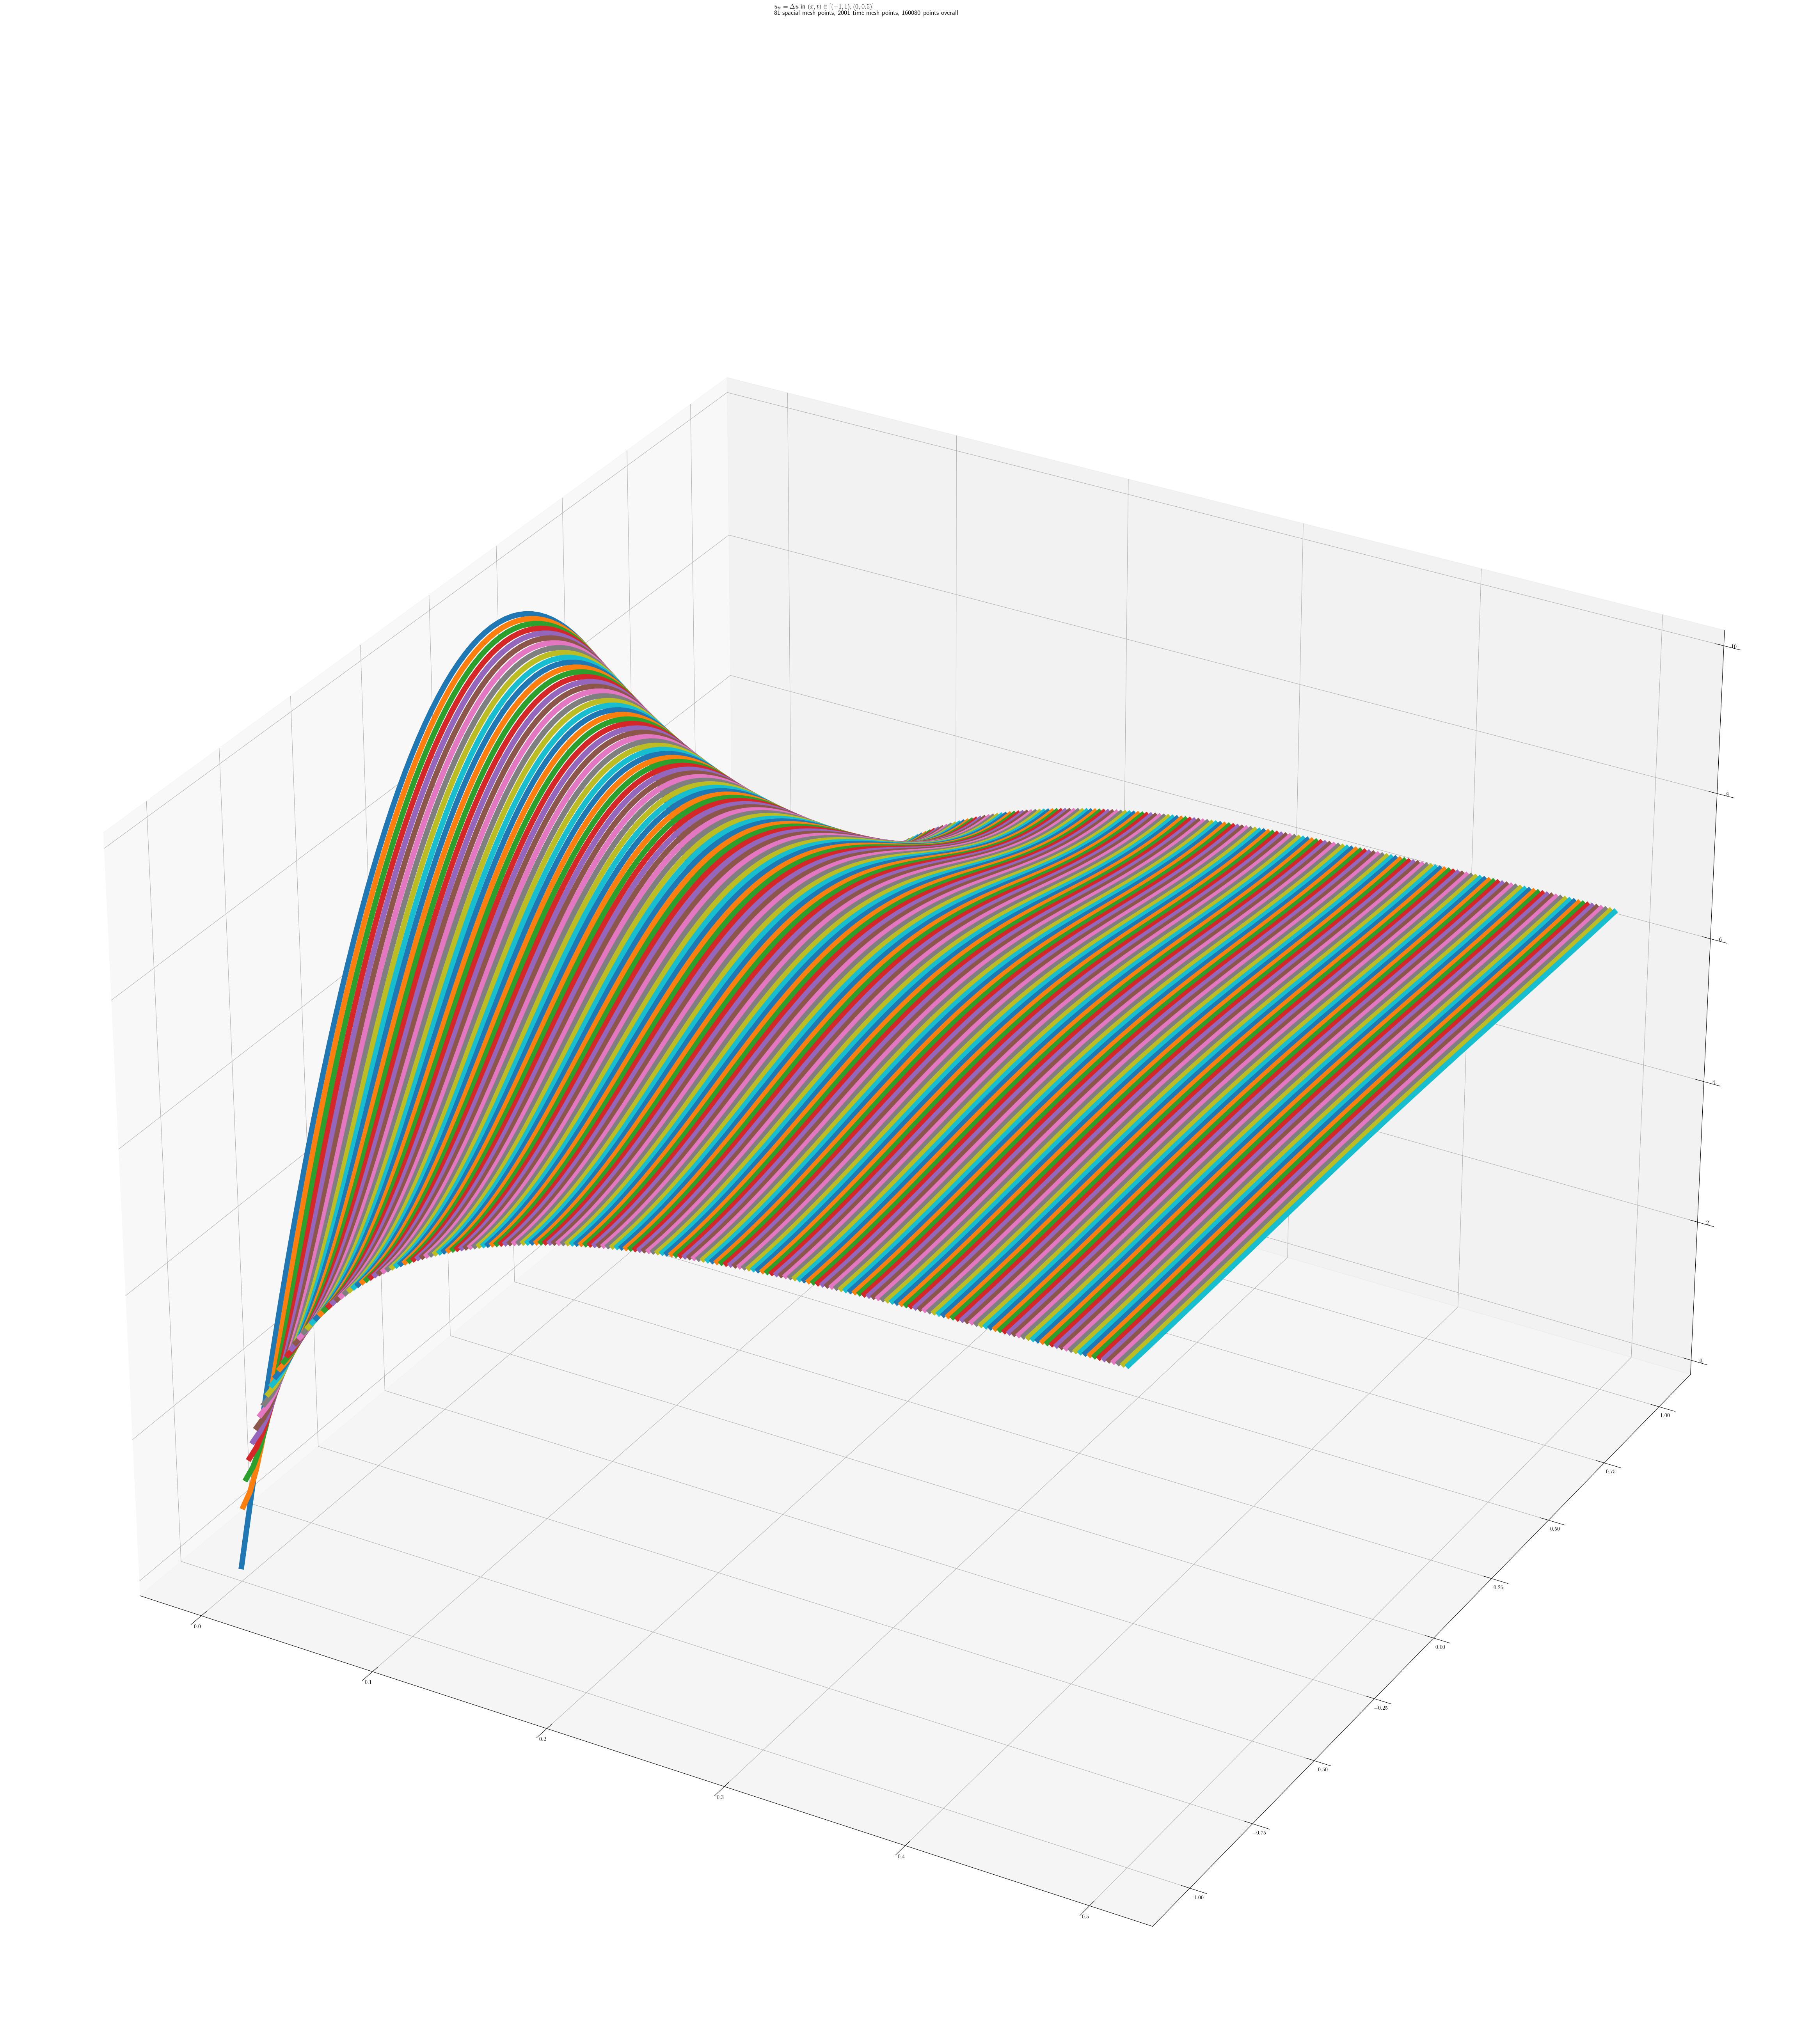
\includegraphics[scale=0.05]{gf}
        \caption{Solution to $L^2$ Gradient Flow Equation for Dirichlet Energy (AKA Heat Equation)}
    \end{figure}
\end{frame}

\begin{frame}
    \frametitle{Dirichlet Gradient Flow in Other Function Space}
    \begin{definition}[Famous Inner Product Function Spaces]
        \begin{itemize}
            \item $L^p = \left\{ f \middle| \left( \int |f|^p \intd x \right)^{1/p} < \infty \right\}$
                \begin{itemize}
                    \item $\inner{f, g}_{L^2} = \int f g \intd x$
                \end{itemize}
            \item $p=2$ Sobolev Space $H^{k} = \left\{ f \middle| \sum_{i=0}^{k} \int \left| \mathcal{D}^{(i)} f \right|^2 \intd x < \infty \right\}$
                \begin{itemize}
                    \item $\inner{f, g}_{H^k} = \sum_{i=0}^k \inner{\mathcal{D}^{(i)} f, \mathcal{D}^{(i)} g}_{L^2}$
                    \item For our case, sufficient to take $\inner{f, g}_{H^k} = \inner{\mathcal{D}^{(k)} f, \mathcal{D}^{(k)} g}_{L^2}$
                \end{itemize}
        \end{itemize}
    \end{definition}

    \onslide<2->
    {
        \begin{itemize}
            \item $L^2 = H^0$: $\frac{\partial f}{\partial t} = - \laplace f$
            \item $H^1$: $\frac{\partial f}{\partial t} = -f$
            \item $H^{-1}$: $\frac{\partial f}{\partial t} = - \laplace^2 f$
                \begin{itemize}
                    \item $\inner{f, g}_{H^{-1}} = \inner{\laplace^{-1} f, \laplace^{-1} g}_{H^1}$
                \end{itemize}
            \item $H^2$: $\frac{\partial f}{\partial t} = \laplace^{-1} f$
        \end{itemize}
    }
\end{frame}

\section{Curve Repulsion}
\begin{frame}
    \frametitle{Gradient Flow on Tangent-Point Energy}
    We now take the tangent-point energy and gradient flow together:
    \begin{equation}
        \frac{\partial \gammabf}{\partial t} = - \grad_{L^2} \mathcal{E}
    \end{equation}
    with $\left.\gammabf\right|_{t=0}$ is the tangled curve.

        \begin{multicols}{2}
            \onslide<2->
            {
                For numerical solution, one discretises the curve.
            }
            \onslide<3->
            {
                Enumerate each point as $\xbf_0, \xbf_1, \cdots, \xbf_{J-1}$, and write
                $\Gammabf$ for the resulting polygonal curve.
            }
            \columnbreak
            \onslide<2->
            {
                \begin{figure}[h]
                    \centering
                    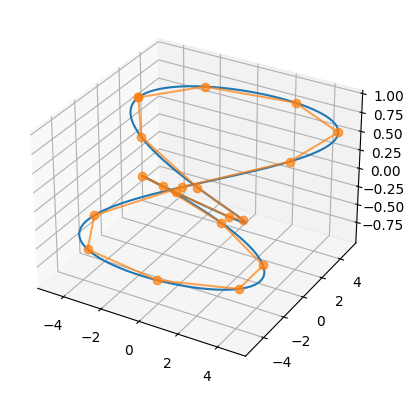
\includegraphics[scale=0.4]{discretization}
                    \caption{Discretised Curve}
                \end{figure}
            }
        \end{multicols}
\end{frame}

\begin{frame}
    \frametitle{Subtlety}
    \begin{figure}[h]
        \centering
        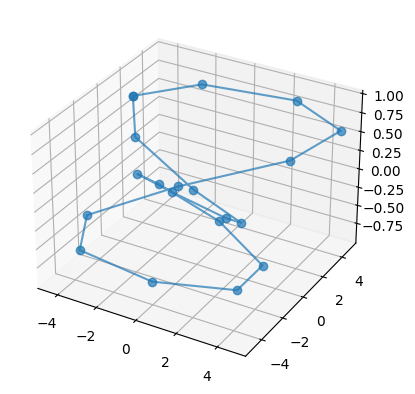
\includegraphics[scale=0.5]{discretization-only}
        \caption{Tangent-point energy is not well-defined for polygonal curves.}
    \end{figure}
\end{frame}

\begin{frame}
    \frametitle{Energy Discretisation}
    Note the form of tangent-point energy:
        \begin{equation}
            \mathcal{E}_{\beta}^{\alpha} \left( \gammabf \right) \coloneqq \iint_{M^2} k_{\beta}^{\alpha} \left( \gammabf_x, \gammabf_y, \mathbf{T}_x \right) \intd \gamma_x \intd \gamma_y
        \end{equation}

    \begin{definition}[Discretised Energy]<2->
        Given a closed curve with discretised points $\xbf_0, \xbf_1, \cdots, \xbf_{J-1}$,
        define \textbf{discretised energy} $E$ as:
        \begin{equation*}
            E \left( \Gammabf \right) \coloneqq \sum_{\substack{i, j \in \left\{ 0, 1, \cdots, J-1 \right\} \\ \dist_{\text{geodesic}} \left( \Gammabf(i), \Gammabf(j) \right) > 1}} 
            %\frac{\norm{\mathbf{T}_x \wedge \left( \gammabf_x - \gammabf_y \right)}^{\alpha}}{\norm{\gammabf_x - \gammabf_y}^{\beta}}
            k_{i,j}
            \norm{\xbf_{i+1} - \xbf_{i}} \, \norm{\xbf_{j+1} - \xbf_{j}}
        \end{equation*}
        where the discretised kernel $k_{i,j}$ is given by:
        \begin{equation*}
            \frac{1}{4} \left( 
                k_{\beta}^{\alpha} \left( x_i, x_j, T_i \right)
                + k_{\beta}^{\alpha} \left( x_i, x_{j+1}, T_i \right)
                + k_{\beta}^{\alpha} \left( x_{i+1}, x_j, T_i \right)
            + k_{\beta}^{\alpha} \left( x_{i+1}, x_{j+1}, T_i \right) \right)
        \end{equation*}
    \end{definition}
\end{frame}

\begin{frame}
    \frametitle{Numerical Scheme}
    Original $L^2$ Gradient Flow Equation:
    \begin{equation}
        \frac{\partial \gammabf}{\partial t} = - \grad_{L^2} \mathcal{E} - \underbrace{\mathcal{C}}_{\text{Constraint}}
    \end{equation}
    By forward difference, we arrived at an explicit Euler scheme:
    \begin{equation*}
        \frac{\Gammabf^{k+1} - \Gammabf^k}{\Delta T} = - \underbrace{\frac{\partial E}{\partial \Gammabf}}_{\text{Gradient from perturbing each point in each direction}}
        - \underbrace{\frac{\partial \mathcal{C}}{\partial \Gammabf}}_{\text{Deriven from Constraint}}
    \end{equation*}
    where we may further approximate the RHS by central difference scheme, for example:
    \begin{equation*}
        \frac{\partial E}{\partial \Gammabf_i} \approx \frac{E|_{\xbf_i += h} - E|_{\xbf -= h}}{2h} \left(= \frac{\partial E}{\partial \Gammabf_i} + O(h^2) \right) 
    \end{equation*}
\end{frame}

\begin{frame}
    \frametitle{Gradient Flow Demo}
    \begin{itemize}
        \item \href{run:./demos/ellipse.mp4}{Ellipse to Circle (ellipse.mp4)}
        \item \href{run:./demos/saddle.mp4}{Saddle to Circle (saddle.mp4)}
    \end{itemize}
\end{frame}

\begin{frame}
    \frametitle{Bibliography}
    \printbibliography
\end{frame}

\end{document}
